\documentclass[a4paper, oneside, final]{scrartcl} 
\usepackage[margin=1in]{geometry}
\usepackage{titlesec} % Allows creating custom \section's
\usepackage{graphicx}
\usepackage{lipsum}
\usepackage{scrpage2} % Provides headers and footers configuration
\usepackage{marvosym} % Allows the use of symbols
\usepackage{tabularx,colortbl} % Advanced table configurations
\usepackage{hyperref}
\usepackage{booktabs}
\usepackage{ltablex}
\usepackage[utf8]{inputenc}

\titleformat{\section}{\Large\scshape\raggedright}{}{0em}{}[\titlerule] % Section formatting

\pagestyle{scrheadings} % Print the headers and footers on all pages

\addtolength{\voffset}{-0.5in} % Adjust the vertical offset - less whitespace at the top of the page
\addtolength{\textheight}{3cm} % Adjust the text height - less whitespace at the bottom of the page

\newcommand{\gray}{\rowcolor[gray]{.90}} % Custom highlighting for the work experience and education sections
\newcommand\YUGE{\fontsize{30}{60}\selectfont}

\begin{document}

\pagenumbering{gobble}% Remove page numbers (and reset to 1)

%\begin{flushleft}
\begin{center}
\YUGE \textsc{Diego Bruciaferri}\\
\end{center}
\bigskip%\bigskip
\textsc{Met Office Hadley Centre}, \hspace{3.2cm} \textsc{E-mail}: \href{mailto:diego.bruciaferri@metoffice.gov.uk}{diego.bruciaferri@metoffice.gov.uk}\\
FitzRoy Road, Exeter, \hspace{7.5cm} \textsc{mobile}: +44 7490 444 958\\
Devon, EX1 3PB \hspace{9.4cm} \textsc{Citizenship}: Italian\\
United Kingdom \hspace{7.6cm} \url{https://github.com/oceandie}\\
%\end{flushleft}
%\begin{center}
%\noindent\rule{6cm}{1.8pt}\\
%\end{center}
%\vspace{0.cm}
%-----------------------------------------------------------------------------------------------------

\section{Research interests}
\normalsize
\noindent
I am a physical oceanographer and ocean modeller interested in understanding the mechanisms underpinning the turbulent multi-scale dynamics of the oceans and how to improve their representation in numerical ocean models. My research interests include the ocean models' representation of the influence of the bottom topography on the oceanic flow, accurate numerical schemes for generalised vertical coordinates (e.g. schemes for computing horizontal pressure forces) and the interplay between the shelf seas and the deep ocean and how to represent the coastal dynamics in large scale coarse models.
%I am a physical oceanographer interested in understanding the mechanisms underpinning the turbulent multi-scales dynamics of the oceans and how to improve their representation in numerical ocean models. I am particularly interested in meso- and sub-mesoscale physical processes, including for example the influence of the bottom topography on the oceanic flow and the interaction between ocean currents and wind-waves. My research involves using and contributing to develop numerical models able to realistically simulate the physical processes of the oceans as well as analysing observations. 
%-------------------------------------------------------------------------------------------------------

\section{Education}
\normalsize
\noindent

\label{tab:daypack}
\begin{tabularx}{\linewidth}{>{\raggedright\scshape}p{4.4cm}|X}
\gray Degree:       & \textbf{Ph.D. in Physical Oceanography}\\
Period:       & \textbf{2015 --- 2020}\\[6pt]
University:   & \textsc{University of Plymouth}, Plymouth, United Kingdom\\
Thesis Title: & \textit{Advanced methods for numerical modelling of regional seas}\\[3pt]
Supervisors:  & \textbf{1st}: Prof. Georgy Shapiro (University of Plymouth, UK)\\
              & \textbf{2nd}: Prof. Tal Ezer (Old Dominion University, USA)\\
              & \textbf{3rd}: Dr.   Fred Wobus (University of Plymouth, UK)\\
\end{tabularx}

%\medskip

\begin{tabularx}{0.97\linewidth}{>{\raggedright\scshape}p{4.4cm}|X}
\gray Degree:       & \textbf{M.Sc. in Environmental Sciences} \\
Period:       & \textbf{2011 --- 2014}\\
%Rank:         & $110/110$, with distinction (\textit{magna cum laude})\\
University:   & \textsc{University of Bologna}, Bologna, Italy\\
Thesis Title: & \textit{Study of a wind-wave numerical model and its integration with an ocean and an oil-spill numerical models}\\[3pt]
Supervisors:  & \textbf{1st}: Prof. Nadia Pinardi (University of Bologna, Italy)\\
              & \textbf{2nd}: Dr. Michela De Dominicis (Instituto Nazionale di Geofisica e Vulcanologia, Italy)\\
\end{tabularx}

%\medskip

\begin{tabularx}{0.97\linewidth}{>{\raggedright\scshape}p{4.4cm}|X}
\gray Degree:       & \textbf{B.Sc. in Marine Sciences} \\ %and Physical Oceanography} \\
Period:       & \textbf{2007 --- 2011}\\
%Rank:         & $100/110$ \\
University:   & \textsc{Polytechnic University of Marche}, Ancona, Italy\\
Thesis Title: & \textit{Implementation of an ocean numerical model to study the dispersion dynamics, in the marine environment, of a cooled and chlorinated seawater discharge coming from a LNG-FSRU terminal}\\[3pt]
Supervisor    & \textbf{1st}: Dr. Aniello Russo (Polytechnic University of Marche, Italy)\\
\end{tabularx}
\pagebreak
%-------------------------------------------------------------------------------------------------------

\section{Professional Appointments}
\noindent
\normalsize
\begin{tabularx}{0.97\linewidth}{>{\raggedright\scshape}p{4.4cm}|X}
	\gray \textsc{Research Title:} & \textbf{Senior Scientist}\\
	\textsc{Period:}               & \textbf{Nov 2021 -- present}\\
	\textsc{Employer:}             & \textsc{Met Office Hadley Centre}, Exeter, UK \\
	\textsc{Group:}                & Ocean Modelling \\%(Manager: Dr. Helene T. Hewitt) \\
	& \\
	\textsc{Main activities}       & \textbf{Ocean model developer} \\
	\textsc{and responsibilities:} & $\bullet$ Development of localised quasi-Eulerian general vertical coordinates to improve the representation of flow-topography interactions (e.g. overflows, boundary currents) and coastal dynamics in global numerical ocean models;\\
	& $\bullet$ Development of numerical schemes to accurately compute pressure forces in ocean models employing generalised vertical coordinates; \\
	
\end{tabularx}
	
\begin{tabularx}{0.97\linewidth}{>{\raggedright\scshape}p{4.4cm}|X}
\gray \textsc{Research Title:} & \textbf{Scientist}\\
\textsc{Period:}               & \textbf{Aug 2019 -- Nov 2021}\\
\textsc{Employer:}             & \textsc{Met Office}, Exeter, UK  \\
\textsc{Group:}                & Shelf seas forecasting \\%(Manager: Dr. Marina Tonani) \\
                               & \\
\textsc{Main activities}       & \textbf{Ocean modelling - R{\&}D} \\
\textsc{and responsibilities:} & $\bullet$ Development of a high resolution ocean model of the Arabian/Persian Gulf area;\\
                               & $\bullet$ Development, analysis and assessment of the ocean-wave coupled forecasting system of the North West European shelf at 1.5 km of resolution;\\
\end{tabularx}

\begin{tabularx}{0.97\linewidth}{>{\raggedright\scshape}p{4.4cm}|X}
\gray \textsc{Research Title:} & \textbf{Senior Ocean Modeller}\\
\textsc{Period:}               & \textbf{Jun 2019 -- Jul 2019}\\
\textsc{Employer:}             & \textsc{University of Plymouth}  \\
                               & \textsc{Plymouth Ocean Forecasting Centre}, Plymouth, UK (Supervisor: Prof. G.I.~Shapiro) \\
                               & \\
\textsc{Main activities}       & \textbf{Ocean model development} \\
\textsc{and responsibilities:} & Development of a high resolution ocean model of the Arabian/Persian Gulf and implementation and testing of several types of lateral boundary conditions.\\
\end{tabularx}

\begin{tabularx}{0.97\linewidth}{>{\raggedright\scshape}p{4.4cm}|X}
\gray \textsc{Research Title:} & \textbf{Ph.D. Researcher}\\
\textsc{Period:}         & \textbf{Oct 2015 -- May 2019}\\
\textsc{Employer:}             & \textsc{University of Plymouth}  \\
                               & \textsc{Coastal Processes Research Group} and \\
                               & \textsc{Plymouth Ocean Forecasting Centre}, Plymouth, UK (Supervisor: Prof. G.I.~Shapiro)\\
                               & \\
\textsc{Main activities}       & $\bullet$ \textbf{Teaching assistant} for the following modules:\\
\textsc{and responsibilities:} & \ \ $\ast$ \textsc{Shelf Seas and Estuaries} (B.Sc.)\\
                               & \ \ $\ast$ \textsc{Introduction to Ocean Modelling} (B.Sc.)\\
                               & \ \ $\ast$ \textsc{Modelling Marine Processes} (M.Sc.)\\
                               & $\bullet$ \textbf{Scientific responsible} for \textbf{EMODnet/Black Sea Checkpoint} -- Coast  \url{http://emodnet-blacksea.eu/}) \\
                               
\end{tabularx}

\newpage

\begin{tabularx}{0.97\linewidth}{>{\raggedright\scshape}p{4.4cm}|X}
\gray \textsc{Research Title:}  & \textbf{Senior Ocean Modeller}\\
\textsc{Period:}          & \textbf{Sep 2017 -- Mar 2018}\\
\textsc{Employer:}        & \textsc{University of Plymouth} \\
                          & \textsc{Plymouth Ocean Forecasting Centre}, Plymouth, UK (Supervisor: Prof. G.I.Shapiro)\\
                                & \\
\textsc{Main activities}        & \textbf{Ocean Modeller} for \textbf{Institutional Links STREAM} \\
\textsc{and responsibilities:}  & \textbf{2016 Grant} - \textit{Physical mechanisms which control water budget and sea level in the Dead Sea}, \url{https://isramar.ocean.org.il/isramar2009/TheBritishCouncil/}. \\
\end{tabularx}
%\pagebreak
%\medskip

\begin{tabularx}{0.97\linewidth}{>{\raggedright\scshape}p{4.4cm}|X}
\gray \textsc{Research Title:}  & \textbf{Research Assistant}\\
\textsc{Period:}          & \textbf{2014 -- 2015}\\
\textsc{Employer:}        & \textsc{Istituto Nazionale di Geofisica e Vulcanologia} (INGV), Bologna, Italy\\
                          & \\
\textsc{Main activities}  & $\bullet$ Research and development of MEDSLIK-II oil spill model (open source model, \url{http://medslikii.bo.ingv.it/}) \\                                 
                          & $\bullet$ Research and development of the SURF (Structured Unstructured Relocatable model for Forecasting) wind-wave module %in collaboration with the SiNCEM (Laboratorio di Simulazioni Numeriche del Clima e degli Ecosistemi Marini - Laboratory of Numerical Simulations of Climate and Marine Ecosystems) research group of the Alma Mater Studiorum University of Bologna. \\
\end{tabularx}          

%-----------------------------------------------------------------------------------
\section{External professional activities}
\noindent
\normalsize
\begin{tabularx}{0.97\linewidth}{>{\raggedright\scshape}p{4.4cm}|X}
	\textbf{2020 -- present}  & Member of the UK \textbf{Joint Marine Modelling Program} (JMMP)\\
\end{tabularx}
\begin{tabularx}{0.97\linewidth}{>{\raggedright\scshape}p{4.4cm}|X}
	\textbf{2020 -- present}  & Member of the \textbf{NEMO} ocean model development group (\textbf{NEMO-KERNEL} working group) \\
\end{tabularx}
\begin{tabularx}{0.97\linewidth}{>{\raggedright\scshape}p{4.4cm}|X}
	\textbf{2014 -- 2015}  & Member of the \textbf{NEMO} ocean model development group (\textbf{NEMO-WAVE} working group) \\
\end{tabularx}

%-----------------------------------------------------------------------------------
%\section{Mentoring}
%\noindent
%\normalsize
%\begin{itemize}
%	\item Ihor Hromov, Ph.D. student, University of Plymouth, UK,  Advisory Committee (since 2020)
%\end{itemize}	

%-----------------------------------------------------------------------------------
\section{Service activities}
\noindent
\normalsize
\begin{itemize}
	\item Member of \textbf{CLIVAR Ocean Model Development Panel} (OMDP; since 2023)
	\item \textbf{Young editorial board member} of Ocean Modelling journal (since 2022)
	\item \textbf{Reviewer} for \textit{Ocean Modelling} (OM), \textit{Ocean Science} (OS) and \textit{Journal of Marine Science and Engineering} (JMSE).
\end{itemize}
%-----------------------------------------------------------------------------------
\section{Fellowships and Awards}
\noindent
\normalsize
\begin{tabularx}{0.97\linewidth}{>{\raggedright\scshape}p{4.4cm}|X}
	\textbf{Feb 2010}  & \textbf{BSc thesis bursary} offered by Ancona province government \\
\end{tabularx}

\begin{tabularx}{0.97\linewidth}{>{\raggedright\scshape}p{4.4cm}|X}
	\textbf{Feb 2019}  & \textbf{PlyMSEF Grant-In-Aid} offered by Plymouth Marine Science and Education Foundation (PlyMSEF) \\
\end{tabularx}



%-----------------------------------------------------------------------------------
\section{Publications}
\noindent
\normalsize
%\textbf{In preparation}
%\begin{itemize}
    
%\end{itemize}

%\noindent
\textbf{Submitted}
\begin{itemize}
\item \textbf{Bruciaferri, D.}, Guiavarc'h, C., Hewitt, H.T., Harle, J., Almansi, M., Mathiot, P. \textit{Localised general vertical coordinates for quasi-Eulerian ocean models: the Nordic overflows test-case} - \textit{in review for} Journal of Advances in Modelling Earth Systems, \url{https://doi.org/10.22541/essoar.168771422.22225431/v1}	
\end{itemize}	
\noindent
\textbf{Peer-reviewed}
\begin{itemize}
\item Jackson, L. C., Hewitt, H. T., \textbf{Bruciaferri, D.}, Calvert, D., Graham, T., Guiavarc’h, C., Menary, M.B., New, A. L., Roberts, M. and Storkey, D. \textit{Challenges simulating the AMOC in climate models}, Phil. Trans. R. Soc. A. 381:20220187, \url{https://doi.org/10.1098/rsta.2022.0187}, 2023	
\item Polton, J., Harle, J., Holt, J., Katavouta, A., Partridge, D., Jardine, J., Wakelin, S., Rulent, J., Wise, A., Hutchinson, K., Byrne, D., \textbf{Bruciaferri, D.}, O'Dea, E., De Dominicis, M., Mathiot, P., Coward, A., Yool, A., Palmiéri, J., Lessin, G., Mayorga-Adame, C.G., Le Guennec, V., Arnold, A. \textit{Reproducible and Relocatable Regional Ocean Modelling: Fundamentals and practices} - Geosci. Model Dev., \url{https://doi.org/10.5194/gmd-16-1481-2023}, 2023
\item \textbf{Bruciaferri, D.}, Tonani, M., Ascione, I., Al Senafi, F., O'Dea, E., Hewitt, H. T., and Saulter, A. \textit{GULF18, a high-resolution NEMO-based tidal ocean model of the Arabian/Persian Gulf}, Geosci. Model Dev., \url{https://doi.org/10.5194/gmd-15-8705-2022}, 2022.
\item Wise, A., Harle, J., \textbf{Bruciaferri, D.}, O'Dea, E., Polton, J. \textit{The effect of vertical coordinates on the accuracy of a shelf sea model}. Ocean Modelling, 170, 101935. \url{https://doi.org/10.1016/j.ocemod.2021.101935}.	
\item \textbf{Bruciaferri, D.}, Tonani, M., Lewis, H. W., Siddorn, J., Saulter, A., Castillo, J. M., Valiente, N. G., Conley, D., Sykes, P., Ascione, I., McConnell, N. \textit{The impact of ocean-wave coupling on the upper ocean circulation during storm events}. Journal of Geophysical Research: Oceans, 126, e2021JC017343. \url{https://doi.org/10.1029/2021JC017343}.
\item Valiente, N. G., Saulter, A., Edwards, J. M., Lewis, H. W., Castillo, J. M., \textbf{Bruciaferri, D.}, Bunney, C., Siddorn, J. \textit{The impact of wave model source terms and coupling strategies to rapidly developing waves across the North-west European Shelf during extreme events}. Journal of Marine Science and Engineering. 2021; 9(4):403. \url{https://doi.org/10.3390/jmse9040403}	
\item \textbf{Bruciaferri, D.}, Shapiro, G., Stanichny, S., Zatsepin, A., Ezer, T., Wobus, F., Francis, X., Hilton, D. \textit{The development of a 3D computational mesh to improve the representation of dynamic processes: the Black Sea test case}, Ocean Modelling, 146 (2020), 101534, \url{https://doi.org/10.1016/j.ocemod.2019.101534}
\item \textbf{Bruciaferri, D.}, Shapiro, G.I. and Wobus, F. (2018) \textit{A multi-envelope vertical coordinate system for numerical ocean modelling}. Ocean Dynamics, Volume 68(10), Pages 1239-1258, \url{https://doi.org/10.1007/s10236-018-1189-x}  
\item M. De Dominicis, \textbf{D. Bruciaferri}, R. Gerin, N. Pinardi, P.M. Poulain, P. Garreau, G. Zodiatis, L. Perivoliotis, L. Fazioli, R. Sorgente, C. Manganiello, \textit{A multi-model assessment of the impact of currents, waves and wind in modelling surface drifters and oil spill}, Deep Sea Research Part II: Topical Studies in Oceanography, Volume 133, November 2016, Pages 21-38, ISSN 0967-0645, \url{https://doi.org/10.1016/j.dsr2.2016.04.002} 
\item F. Trotta, E. Fenu, N. Pinardi, \textbf{D. Bruciaferri}, L. Giacomelli, I. Federico, G. Coppini, \textit{A Structured and Unstructured grid Relocatable ocean platform for Forecasting (SURF)}, Deep Sea Research Part II: Topical Studies in Oceanography, Volume 133, November 2016, Pages 54-75, ISSN 0967-0645, \url{https://doi.org/10.1016/j.dsr2.2016.05.004}
%\pagebreak
\item G. Zodiatis, M. De Dominicis, L. Perivoliotis, H. Radhakrishnan, E. Georgoudis, M. Sotillo, R.W. Lardner, G. Krokos, \textbf{D. Bruciaferri}, E. Clementi, A. Guarnieri, A. Ribotti, A. Drago, E. Bourma, E. Padorno, P. Daniel, G. Gonzalez, C. Chazot, V. Gouriou, X. Kremer, S. Sofianos, J. Tintore, P. Garreau, N. Pinardi, G. Coppini, R. Lecci, A. Pisano, R. Sorgente, L. Fazioli, D. Soloviev, S. Stylianou, A. Nikolaidis, X. Panayidou, A. Karaolia, A. Gauci, A. Marcati, L. Caiazzo, M. Mancini, \textit{The Mediterranean Decision Support System for Marine Safety dedicated to oil slicks predictions}, Deep Sea Research Part II: Topical Studies in Oceanography, Volume 133, November 2016, Pages 4-20, ISSN 0967-0645, \url{https://doi.org/10.1016/j.dsr2.2016.07.014}
\end{itemize}
%\pagebreak
%-------------------------------------------------------------------------------------------------------
\section{Selected Conferences and Talks}
\noindent
\normalsize
\begin{itemize}
\item \textbf{Bruciaferri, D.}, Hewitt, H.T., Bell, M.J., Guiavarc'h, C., Storkey, D., Roberts, M.J. and Jackson, L. \textit{Sensitivity of the Western North Atlantic circulation to the vertical coordinate system in global ocean models}. `Whither the Gulf Stream' Workshop - Woods Hole, MA, USA, June 2022.
%\item \textbf{Bruciaferri, D.}, Guiavarc'h, C., Hewitt, H., Harle, J., Almansi, M., and Mathiot, P. \textit{Improving nordic overflows representation in global ocean models}, EGU General Assembly 2022, Vienna, Austria, 23–27 May 2022, EGU22-4072	
\item Bell, M.J. and \textbf{Bruciaferri, D.} \textit{Accurate calculation of pressure forces on cells defined by steeply sloping coordinates}, EGU General Assembly 2022, Vienna, Austria, 23–27 May 2022, EGU22-5012. 
\item \textbf{Bruciaferri, D.}, Harle, J., Wise, A., O'Dea, E. and Polton, J.  \textit{The impact of the vertical discretization scheme on the accuracy of a model of the European north-west shelf}. EGU General Assembly 2021, EGU21-4152, April 2021.
%\item \textbf{Bruciaferri, D.}, Tonani, M., Lewis, H.W., Siddorn, J., King, R.R., Sykes, P., Castillo, J.M., Saulter, A., McConnell, N., Ascione, I., and O'Dea, E.  \textit{Modelling the upper ocean dynamics of the north-west European shelf during storm events with the UK Met Office ocean-wave prediction system}. Geophysical Research Abstracts. Vol. 22, EGU2020-4960, May 2020.
\item \textbf{Bruciaferri, D.} \textit{A Multi Envelope $s$-coordinate system for numerical ocean modelling: idealised and realistic experiments}, Department of Physics, University of Oxford, 29$^{th}$ January 2020, Oxford (UK) (\textit{Invited}). 
%\item \textbf{Bruciaferri, D.}, Shapiro, G., Stanichny, S., Zatsepin, A., Ezer, T., Wobus, F., Francis, X. and Hilton, D. \textit{A new numerical model for the Black Sea circulation}. Geophysical Research Abstracts. Vol. 21, EGU2019-5933, 2019, April 2019.
\item \textbf{D. Bruciaferri}, G. Shapiro, S. Stanichny, A. Zatsepin, T. Ezer, F. Wobus, X. Francis and D. Hilton. \textit{A numerical model of the Black Sea circulation using a structured multi-envelope mesh with variable resolution}. Met Office seminars, $5^{th}$ March 2019, Exeter (UK) (\textit{Invited}).
%\item \textbf{D. Bruciaferri}, G. Shapiro, S. Stanichny, A. Zatsepin, T. Ezer, F. Wobus, X. Francis and D. Hilton. \textit{An advanced numerical model of the Black Sea}. PlyMSEF conference, Plymouth Marine Laboratory, $5^{th}$ February 2019, Plymouth (UK) (\textit{Oral}).
%\item G. I. Shapiro, R. Manasrah, I. Gertman and \textbf{D. Bruciaferri}. \textit{The effect of different types of water column structure on the sea level in the Dead Sea}. Geophysical Research Abstracts. Vol. 20, EGU2018-19780, April 2018 (\textit{Poster}).
\item \textbf{Bruciaferri, D.}, Shapiro, G.I. and Wobus, F. \textit{An Advanced Vertical Coordinate System to Improve the Representation of the Oceanic Transport in Regional Non-Isopycnal Ocean Models}. Abstract 310863 presented at 2018 Ocean Sciences Meeting, Portland, OR, 12-16 February 2018.
%\item \textbf{Bruciaferri, D.}, Shapiro, G.I. and Wobus, F. \textit{The development of an advanced vertical discretisation scheme for a regional ocean model}. Geophysical Research Abstracts. Vol. 19, EGU2017-7276, April 2017.
%\item \textbf{D. Bruciaferri}, G. I. Shapiro, F. Wobus, \textit{A coupled ocean-wave modeling system to investigate the role of the wave-induced turbulence on the Cold Intermediate Water formation in the Black Sea - The scientific approach}, NPOP conference, Bristol (UK), April 2016 (\textit{Poster}).
%\item M. De Dominicis, N. Pinardi, \textbf{D. Bruciaferri}, S. Liubartseva, \textit{Numerical modelling for real-time forecasting of marine oil pollution and hazard assessment}, EGU assembly 2015.
\end{itemize}
%\pagebreak
%-------------------------------------------------------------------------------------------------------
%\section{Technical Reports}
%\noindent
%\normalsize
%\begin{itemize}
%\item B. B. Romain, P. A. Bouttier, C. Bricaud, \textbf{D. Bruciaferri}, J. Chanut, S. A. Ciliberti, E. Clementi, A. Coward, D. Delrosso, C. Ethé, S. Flavoni, T. Graham, J. Harle, D. Iovino, D. Lea, C. Lévy, T. Lovato, G. Madec, N. Martin, S. Masson, P. Mathiot, S. Mocavero, G. Nurser, E. O’Dea, J. Paul, C. Rousset, D. Storkey, A. Storto, 2016, \textit{Main achievements for NEMO evolution during MyOcean period}, Mercator Ocean Journal, 54
%\item \textbf{D. Bruciaferri} and the MEDSLIK-II System Team, 2016. MEDSLIK-II, \textit{Lagrangian marine surface oil spill model, User Manual, Version 1.02}.\\
%\end{itemize}
%-----------------------------------------------------------------------------------

\section{Specialised Education}
\noindent
\normalsize
%\begin{tabularx}{0.97\linewidth}{>{\raggedright\scshape}p{4.4cm}|X}
%\gray PG Course: & \textbf{Foundation Meteorology}\\
%Period:          & \textbf{March-April 2020}\\
%Institute:       & \textsc{Met Office College - Met Office} \hfill Exeter, United Kingdom\\
%Lecturers:       & T. Howard, W. Tennant, D. Miles, B. Johnson \\
%\end{tabularx}

\begin{tabularx}{0.97\linewidth}{>{\raggedright\scshape}p{4.4cm}|X}
\gray PG Course: & \textbf{Fluid Dynamics Summer School}\\
Period:          & \textbf{September 2016}\\
Institute:       & \textsc{University of Cambridge} \hfill Cambridge, United Kingdom\\
                 & Department of Applied Mathematics and Theoretical Physics (DAMTP)\\
Lecturers:       & P. Bates, S. Bittlestone, C. Caulfield, J.M. Chomaz, S. Dalziel, P. Haynes, H. Johnson, P. Linden, M. McIntyre, C. Muller, J. Neufeld, S. Ortiz, R. Plougonven, E. Shuckburgh, A. Stegner, J. Taylor, A. Woods, T. Woollings, G. Worster, V. Zeitlin\\
\end{tabularx}

\begin{tabularx}{0.97\linewidth}{>{\raggedright\scshape}p{4.4cm}|X}
\gray PG Course: & \textbf{Ifremer Waves Spring School}\\
Period:          & \textbf{June 2016}\\
Institute:       & \textsc{Institut Universitaire Européen de la Mer (IUEM)} \\
                 & Brest, France\\
Lecturers:       & F. Ardhuin, A. Roland\\
\end{tabularx}

\begin{tabularx}{0.97\linewidth}{>{\raggedright\scshape}p{4.4cm}|X}
\gray PG Course: & \textbf{Introduction to OpenMP and MPI}\\
Period:          & \textbf{December 2015}\\
Institute:       & \textsc{ARCHER at \textsc{University of Portsmouth}}, Portsmouth, United Kingdom\\
\end{tabularx}

\begin{tabularx}{0.97\linewidth}{>{\raggedright\scshape}p{4.4cm}|X}
\gray PG Course: & \textbf{NCEP/UMD Waves Summer School}\\
Period:          & \textbf{June 2015}\\
Institute:       & NCEP and \textsc{University of Maryland}, Washington D.C., USA \\
                 & Department of Atmospheric and Oceanic Science\\
Lecturers:       & J.-H. Alves, A. Chawla, A. van der Westhuysen
\end{tabularx}

\begin{tabularx}{0.97\linewidth}{>{\raggedright\scshape}p{4.4cm}|X}
\gray PG Course:  & \textbf{Advanced Numerical Methods for Hyperbolic Equations and Applications Winter School}\\
Period:           & \textbf{February 2015}\\
Institute:        & \textsc{University of Trento}, \hfill Trento, Italy \\
                  & Department of Civil and Environmental Engineering, \\
                  & Laboratory of Applied Mathematics\\
Lecturers:        & E. Toro and M. Dumbser\\
\end{tabularx}

\begin{tabularx}{0.97\linewidth}{>{\raggedright\scshape}p{4.4cm}|X}
\gray PG Course:       & \textbf{Introduction to Fortran90}\\
Period:                & \textbf{October 2014}\\
Institute:             & \textsc{CiNECA} computing centre, Casalecchio di Reno (Bologna), Italy \\
\end{tabularx}

\begin{tabularx}{0.97\linewidth}{>{\raggedright\scshape}p{4.4cm}|X}
\gray PG Course: & \textbf{Introduction to Python}\\
Period:          & \textbf{September 2014}\\
Institute:       & \textsc{CiNECA} computing centre, Casalecchio di Reno (Bologna), Italy\\
\end{tabularx}
%
\begin{tabularx}{0.97\linewidth}{>{\raggedright\scshape}p{4.4cm}|X}
\gray PG Course: & \textbf{Introduction to HPC Scientific Programming: tools and techniques}\\
Period:          & \textbf{November 2013}\\
Institute:       & \textsc{CiNECA} computing centre, Casalecchio di Reno (Bologna), Italy\\
\end{tabularx}
%
%-------------------------------------------------------------------------------------------------------
\section{Personal skills}
\noindent
\normalsize

\begin{itemize}
\item \textsc{Languages:} Italian (mother tongue), English and Spanish \\

\item \textsc{Computer skills:}
        \begin{itemize}
           \item \textbf{Operating systems}: Unix and Windows based
           \item \textbf{Programming Lannguages}: Fortran77 and 90-95-2003, Python, Matlab, Latex
           \item \textbf{Scripting Languages}: Bash and Shell\\           
        \end{itemize}
\item \textsc{Numerical Models:}
        \begin{itemize}
           \item \textbf{Hydrodynamic models}: NEMO, MITgcm
           \item \textbf{Spectral Wave models}: WW3, SWAN
           \item \textbf{Lagrangian models}: MEDSLIK-II, OpenDrift\\           
        \end{itemize}                 
%\item Open Water PADI license, 01/07/2009
\end{itemize}
%-------------------------------------------------------------------------------------------------------
%\pagebreak
\section{References}
\bigskip
\noindent
\begin{tabularx}{0.97\linewidth}{c|c|c}

\textbf{Prof. Georgy I. Shapiro}      & \textbf{Prof. Tal Ezer}            & \textbf{Prof. Nadia Pinardi}\\
\textit{School of Biological}         & \textit{Center for Coastal}        & \textit{Department of Physics} \\
\textit{and Marine Sciences},         & \textit{Physical Oceanography},    & \textit{and Astronomy} \\
\textsc{University of Plymouth},      & \textsc{Old Dominion University},  & \textsc{University of Bologna},\\
Drake Circus, Plymouth,               & 4111 Monarch Way,                  & Viale Berti Pichat 6, \\ 
PL4 8AA                               & Norfolk, VA 23508                  & 40127, Bologna, Italy \\
+44 (0)1752 584721                    & +1-757-683-5631                    & +39 0544 937324 \\
\href{mailto:G.Shapiro@plymouth.ac.uk}{G.Shapiro@plymouth.ac.uk} & \href{mailto:tezer@odu.edu}{tezer@odu.edu} & \href{mailto:nadia.pinardi@unibo.it}{nadia.pinardi@unibo.it}\\

\end{tabularx}

\begin{center}
\noindent\rule{16.2cm}{1pt}\\
\end{center}
\bigskip

\begin{flushleft}
%\begin{center}
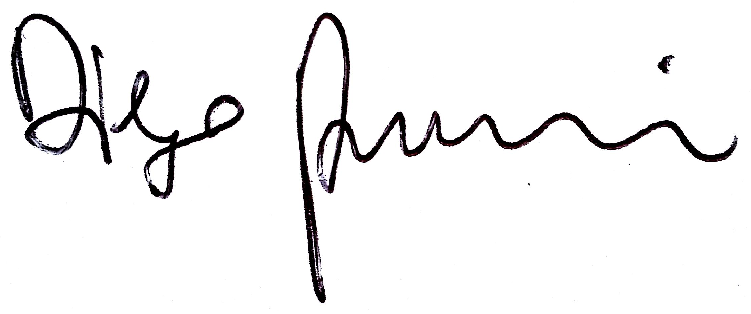
\includegraphics[width=5cm]{./firma_Diego.png}\\
%\end{center}
\end{flushleft}

Diego Bruciaferri \hspace{8cm} \today



\end{document}